\documentclass{book}
\usepackage[utf8]{inputenc}


\usepackage{natbib}
\usepackage{graphicx}
\usepackage{amsmath,amssymb}
\usepackage{ascmac}
\usepackage{braket}
\usepackage{makeidx}
\makeindex
\usepackage{textcomp}
\usepackage{comment}
\usepackage{authblk}

\begin{document}
\title{Lecture Note \\ Quantum Mechanics of Light and Matters}
\author{Yasuyuki Ozeki}
\affil{Department of Electrical Engineering and Information Systems \\ The University of Tokyo}
\date{July 25, 2020}

\maketitle
\tableofcontents
\mainmatter


\chapter{Introduction}
Quantum optics deals with quantum nature of light, where light is regarded as an ensemble of particles called photons. The quantum nature of light appears as `noise' in various applications in optics and photonics such as optical measurement, optical manipulation, and optical communications, leading to the physical limit called quantum limit on the performance or precision achieved by these methods. To push the performance of various methods to the physical limit, it is crucial to understand the quantum limit. Furthermore, quantum nature of light is extensively utilized to develop various quantum technologies such as quantum cryptography, quantum teleportation, and quantum computing. 

Optical measurement always involves the detection of light. It is categorized into direct detection and homodyne/heterodyne detection. Direct detection gives the intensity of light, and homodyne/heterodyne detection which gives the amplitude of light. Furthermore, optical amplification is often utilized before photodetection to mitigate the effect of detector noise. In every case, the signal-to-noise ratio is ultimately limited by quantum noise, and becomes the same order as the number of photons. This limit cannot be surpassed by classical (i.e., non-quantum) methods, while various methods to surpass the limit is developed by using quantum optics.

This lecture note aims at dealing with quantum noise of light. Chapter 2 summarizes the noise in optical measurements. Chapter 3 introduces quantum harmonic oscillators, which is an analogue of light in quantum optics. Chapter 4 describes the evolution of quantum states. Chapter 5 explains the quantization of light. Chapter 6 introduces representative quantum states. Chapter 7 describes two main interactions in quantum optics: mode mixing and parametric amplifications. Chapter 8 explains quantum optical treatment of optical measurements.

This lecture memo was first prepared in Japanese in 2017, in which I referred to Prof. Kazuro Kikuchi's lecture note. Then I rearranged the contents in English in 2020. In particular, I tried to provide an intuitive picture of quantum optics by extensively using wavefunctions. I often hear that quantum optics is abstract; we can somehow calculate various properties of light using bra-ket and operators, while the physics behind them are quite unclear. Instead, typical quantum-optical calculation using operators can be understood as the rotation and distortion of wavefunctions. I hope that this lecture memo provide such intuitive pictures along with the calculation procedures.  I appreciate many comments and feedback from students in my research group and in the lecture. Any feedback is appreciated at \texttt{https://github.com/ysozeki/quantum-optics}.


\chapter{Noise in optical measurement}
This chapter introduces various detection methods of light and explains noise appearing in each method. Some explanations are phenomenological but they will be explained by quantum optics in later chapters.

\section{Optical measurement}
Figure \ref{fig:photodetection}(a) shows the \textbf{direct detection}. Photodetectors can convert photons to electrons to measure optical power, which is proportional to the number of photons per unit time. 

Fig. \ref{fig:photodetection}(b) shows the \textbf{interferometric detection}, where a beamsplitter (BS) is used to mix the signal light wave to be measured and another light wave called local oscillator (LO) light, and the output light waves of the BS are detected with photodetectors to measure the amplitude of light. When the optical frequencies of signal and LO are the same, the method is called \textbf{homodyne}. When they are different, the method is called \textbf{heterodyne}.

Furthermore, an optical amplifier is often used before photodetection as shown in Fig. \ref{fig:photodetection}(c). This is called \textbf{preamplification}. Although not shown in the figure, it is also possible to conduct interferometric detection after preamplification. 

In any case, the output signal of the photodetector contains noise due to various origins such as instability of light sources or optical systems, circuit noise of photodetector(s), and so on. We can somehow reduce these noises, but at last we will see `quantum noise' that cannot be reduced by classical manner. Only quantum optics can control the quantum noise.

Here, before introducing various noise sources, we introduce direct detection, interferometric detection, and preamplification.

\begin{figure}
  \centering
  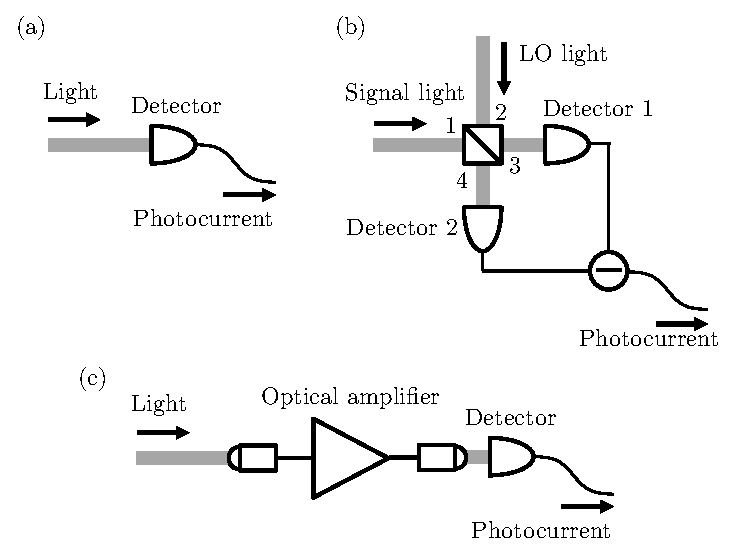
\includegraphics[width=9cm]{fig/2-1_photodetection.eps}
  \caption{Various photodetection methods. (a) Direct detection. (b) Interferometric detection. (c) Optical preamplification with an optical amplifier.}
  \label{fig:photodetection}
\end{figure}


\subsection{Direct detection}
In direct detection, photocurrent $I$ is proportional to the optical power $P$ as 
\begin{equation}
	I = \frac{\eta e P}{\hbar \omega},
	\nonumber
\end{equation}
where $\hbar \omega$ is the photon energy, and $e = 1.602 \times 10^{-19} \ \mathrm{[C]}$ is the elementary charge. $P / \hbar \omega$ is the number of photons incident on the photodetector per unit time. $\eta$ is the quantum efficiency, which is the ratio of the number of photoelectrons and the number of photons.
\footnote{For electrical engineers, it is worth remembering that the photon energy at the optical communication wavelength 1.55 \ \textmu m is approximately 0.8 eV. Since $\hbar \omega / e$ is the photon energy in the unit of eV and typical photodiodes have a quantum efficiency of 90\%, typical conversion efficiency is $I/P \sim 1.1 \mathrm{A/W}$ (see catalogues of InGaAs photodiodes).}

\subsection{Homodyne and heterodyne detection}

\begin{equation}
\begin{aligned}
	a(t) &= \alpha e^{-i(\omega + \Delta \omega)t}\\
  	b(t) &= \beta e^{-i\omega t}
\end{aligned}\label{eq:complex_amplitude}
\end{equation}

\begin{equation}
\begin{aligned}
  a' &= \frac{1}{\sqrt 2}(a - b)\\
  b' &= \frac{1}{\sqrt 2}(a + b)
\end{aligned}\label{eq:BS_complex_amplitude}
\end{equation}

\begin{equation}
  \left( \begin{array}{c}
  	a' \\ b'
  \end{array}
  \right) =
  \frac{1}{\sqrt 2}\left( \begin{array}{r r} 
  	1 & -1 \\ 1 & 1
 \end{array}
	\right)
	\left( \begin{array}{c}
		a \\ b
	\end{array} \right)
	\label{eq:beamsplitter_matrix}
\end{equation}

\begin{equation}
\begin{aligned}
  I_1 &= \frac q \tau |a'|^2 = \frac{q}{\tau}\left|\frac{1}{\sqrt 2} (a - b)\right|^2\\
  I_2 &= \frac q \tau |b'|^2 = \frac{q}{\tau}\left|\frac{1}{\sqrt 2} (a + b)\right|^2
\end{aligned}
\end{equation}

\begin{equation}
\begin{aligned}
  I_2 - I_1 &= \frac{q}{\tau}(ab^* + a^* b)\\
  &= 2qB(\alpha \beta^* e^{-i\Delta\omega t} + \alpha^* \beta e^{i\Delta\omega t})\\
  &= 4qB|\beta|\left\{\mathrm{Re} \  (\alpha e^{-i\phi}) \cos \Delta \omega t + \mathrm{Im} \ (\alpha e^{-i\phi}) \sin \Delta \omega t\right\}
\end{aligned}\label{eq:output_of_balanced_detector}
\end{equation}

Here $B = 1/2\tau$ is the Nyquist frequency, and $\beta = |\beta|e^{i\phi}$.


\section{Noise sources}
\subsection{Shot noise}
\begin{equation}
	p(k) = \frac{\lambda^k e^{-\lambda}}{k!}
\end{equation}

\begin{equation}
\begin{aligned}
	V[p(k)] &= \sum_k{(k-\lambda)^2}p(k)\\
	&= \sum_k{k^2 p(k) - 2\lambda k p(k) + \lambda^2 p(k)} = \sum_k{k^2 p(k) - \lambda^2} \\
	&=\sum_k{k\lambda p(k-1) - \lambda^2} = \lambda\sum_k{\left\{ (k-1)p(k-1) + p(k-1)\right\}}-\lambda^2 \\
	&= \lambda(\lambda + 1) - \lambda^2 = \lambda
\end{aligned}
\end{equation}

\begin{equation}
	\begin{aligned}
		I_{\mathrm{shot}} = q\sqrt{\lambda}/\tau = q\sqrt{\frac{I\tau}{q}}/\tau = \sqrt{\frac{qI}{\tau}}
	\end{aligned}
\end{equation}
\begin{equation}
	\begin{aligned}
		I_\mathrm{shot}=\sqrt{2qIB}
	\end{aligned}
\end{equation}

\begin{equation}
  \mathrm{SNR} = I^2 / I_\mathrm{shot}^2 = I/2qB = 2qB|\alpha |^2/2qB = |\alpha|^2
\end{equation}
where $I=q|\alpha|^2/\tau = 2qB|\alpha|^2$. Since $|\alpha|^2$ corresponds to the number of photons, we can see that the shot-noise limited SNR is equal to the number of photons.


\subsection{Thermal noise}


\subsection{Optical amplifier noise}
\section{Summary}

\chapter{Quantum harmonic oscillators}
\section{Schr\"odinger equation}
\subsection{Wavefunction and energy eigenstates}
\subsection{Fock representation}
\subsection{Position representation}
\subsection{Momentum representation}
\section{Measurement of observables}
\subsection{Expectation value}
\subsection{Expectation of variance}
\section{Multimode quantum states}
\section{Summary}

\chapter{Evolution of quantum states}
\section{Schor\"odinger picture}
\section{Heisenberg picture}
\section{Unitary transformation of quantum states}
\subsection{Time evolution}
\subsection{Displacement}
\subsection{Mode mixing}
\subsection{Single-mode squeezing}
\subsection{Two-mode squeezing}
\section{Summary}

\chapter{Quantization of light}
\section{Mode decomposition of electromagnetic waves}
\subsection{Time-frequency mode}
\subsection{Spatial mode}
\subsection{Polarization}
\section{Operator notation of electromagnetic waves}
\section{Summary}

\chapter{Representative quantum states}
\section{Number states}
\section{Superposition states}
\section{Coherent states}
\section{Squeezed states}
\section{Two-mode squeezed states}
\subsection{EPR state}
\section{Summary}

\chapter{Control of quantum states of light}
\section{Mode mixing}
\subsection{Beamsplitter}
\subsection{Waveplates}
\subsection{Optical loss}
\subsection{Fourier transform}
\section{Parametric amplification}
\subsection{Squeezing}
\subsection{Spontaneous parametric down conversion}
\subsection{Optical amplification}
\subsection{Raman scattering}
\section{Summary}

\chapter{Quantum-optical measurement}
\section{Direct detection}
\section{Homodyne detection}
\section{Heterodyne detection}
\section{Preamplification}
\section{Quantum teleportation}
\section{Summary}

\appendix
\chapter{Appendix}
\section{Bra-ket notation}
\section{Creation and annihilation operators}
\section{Pure states and mixed states}
\section{Wigner function}

\begin{equation}
\begin{aligned}
  \sum_{k=1}^\infty \frac 1 {2^k} &= \frac 1 {2^1} + \frac 1 {2^2} + \frac 1 {2^3} + \dots \\
  &= \frac{1}{2} + \frac{1}{4} + \frac{1}{8} + \dots \\
  &= \frac{\frac 1 2}{1-\frac 1 2} =  1
\end{aligned}
\end{equation}

There is a theory which states that if ever anyone discovers exactly what the Universe is for and why it is here, it will instantly disappear and be replaced by something even more bizarre and inexplicable.
There is another theory which states that this has already happened.

\begin{figure}[h!]
\centering
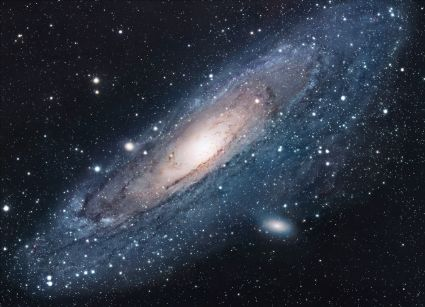
\includegraphics[scale=1.7]{universe}
\caption{The Universe}
\label{fig:universe}
\end{figure}

%\section{Conclusion}
``I always thought something was fundamentally wrong with the universe'' \citep{adams1995hitchhiker}

\bibliographystyle{plain}
\bibliography{references}
\end{document}
